\documentclass{article}
\usepackage{amsmath}
\usepackage{geometry}
\usepackage{float}
\usepackage{graphicx}
\usepackage{fancyref}
\usepackage{hyperref}
\usepackage{enumerate}


\newcommand{\upcite}[1]{\textsuperscript{\cite{#1}}}
\geometry{a4paper,left=2.5cm,right=2.5cm,top=2.5cm,bottom=2.5cm}

\title{Percolation model applied in pandemic research: a cellular automata view}
\author{Xuanzhe Xia\quad Songyu Li\quad Xiangyu Gao}
\begin{document}
\maketitle
\section{Introduction and Motivation}
\subsection{Percolation}
Percolation\upcite{stauffer2018introduction} is a simple yet elegant model in statistical physics that was initially proposed by engineer Simon Broadbent and mathematician John Hammersley in the 1950s.\upcite{broadbent_percolation_1957}. The model was originally inspired by the functioning of activated charcoal gas masks. However, due to its simplicity and applicability to critical phenomena, it has since been used in various complex systems.

The percolation is a simple model on a lattice in which the nodes (sites) or edges (bonds) [respectively called site or bond percolation] are occupied with some probability $p$ or unoccupied with probability $q=1-p$. The example of two dimension square lattice is as fig.\ref{eg1}, where the black square denotes the occupied site, white square denotes the unoccupied site.
\begin{figure}[htbp]
    \label{eg1}
    \centering
    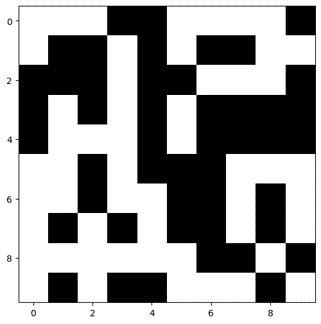
\includegraphics[width=0.4\textwidth]{pic/eg.png}
    \caption{Example of site percolation}
\end{figure}

A system is regraded as percolating if there is a path from one side to the other parallel one, passing only through occupied bonds and sites. This percolation property is only statistically present when the system reaches a critical point denoted as $p_c$.

When percolation reaches its critical point, certain quantities exhibit power law behavior that is analogous to other well-known critical phenomena in physics, such as the superconductivity transition. These critical exponents, which describe the behavior of percolation near its critical point, are identical to those that describe other critical phenomena, such as the Ising model or the superconducting phase transition. This means percolation could be the easiest model to work on studying the whole universality class.

Numerous models have been developed from the basic percolation model, such as directed percolation \upcite{OBUKHOV1980145}, which incorporates a time-varying component into the thermostatistical model, and bootstrap percolation\upcite{ADLER1991453}. These derived models belong to different universality classes, allowing researchers to investigate more complex and practical critical phenomena.

After more than 70 years of research, the threshold of percolation on various lattices has almost been resolved. Currently, an increasing number of researchers are focusing on the practical applications of percolation. For example, Meng. et al. studied a percolation based measurement, the order parameter's abrupt transition to predict a comming El Nino conditions\upcite{meng_percolation_2017}, and Ziff analyzed the spread of an epidemic in 2021.\upcite{ziff_percolation_2021}

% Numerical studies of percolation are straightforward by comparison with many simulations in statistical physics because no Markov process is needed to perform importance sampling.\upcite{newman_efficient_2000}

\subsection{Cellular Automata}
% |TO DO| Need to be completed 

\subsection{Pandemic}
During the past three years, the pandemic has become a major public health threat. As a typical Markovian process, the modeling and estimation of pandemic spreading is mainly worked out by solving PDEs, see \cite{JI20145067} \cite{COOPER2020110057}. However, percolation model point out that if we want to study the critical phenomena near the pandemic spreading threshold, studying the percolating threshold on a certain lattice may be helpful, see in Ziff's recent work\upcite{ziff_percolation_2021}.

However, recent researchers mostly focus on the threshold of SIR (“susceptible-infected-removed”) epidemic model, which involves no time component, since the bond of the percolation model will never be removed.\upcite{araujo_recent_2014} The SIS (“susceptible-infected-susceptible”) model which corresponding to a directed Percolation has yet been detailed studied. Meanwhile, study\upcite{domany_equivalence_1984} has shown the equivalence of cellular automata and a directed percolation, this may be a break point to find out an efficient solution to the threshold of a pandemic.

We will use some derived percolation model to estimate the threshold of a pandemic, and see if the knowledge of cellular automata will either improve our calculation or bring some idea in deriving new percolation models.
\section{Schedule}

\begin{enumerate}[(1)]
    \item We will review the former work of percolation applied on pandemic.
    \item Using computer program to simulate a certain percolation threshold.
    \item Using cellular automata to improve our program.
\end{enumerate}
% |TO DO| 我这Schedule写的什么乱七八糟的
\section{Acknowledgement}
ChatGPT is acknowledged by the authors for modifying the grammar.

\bibliographystyle{unsrt}
\bibliography{percolation}
\end{document}